\documentclass[border=2pt]{standalone}
\usepackage[compat=1.1.0]{tikz-feynman}

\begin{document}
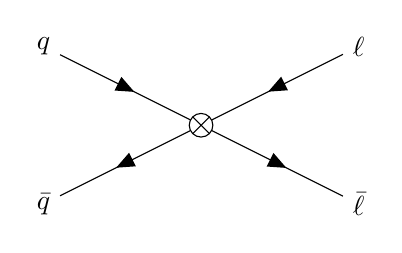
\begin{tikzpicture}
\begin{feynman}
  \vertex (q1) at (0, 1) {\(q\)};
  \vertex (q1bar) at (0, -1) {\(\bar{q}\)};
  \vertex[crossed dot] (c) at (2, 0) {};
  \vertex (l2) at (4, 1) {\(\ell\)};
  \vertex (l2bar) at (4, -1) {\(\bar{\ell}\)};

  \diagram* {
    (q1) -- [fermion] (c) -- [fermion] (q1bar),
    (l2) -- [fermion] (c) -- [fermion] (l2bar),
  };
\end{feynman}
\end{tikzpicture}
\end{document}
